\documentclass{article}
\usepackage{graphicx}
\usepackage{fullpage}
\title{A report on the exam project number 14 - cubic sub-spline for data with derivitives}
\author{A.T.~Hopkinson}
\date{29/06/2021}
\begin{document}
\maketitle

\begin{Abstract}
Introduce the document here
\end{abstract}

\section{Introduction to sub-splines}
Sub-splines are peicewise polynomials but unlike splines do not demand maximal differentiability of the spline. They can therefore do things such as minimize the wiggles and lumps that can be present with other splines. An exampkle of a sub-spline is the Akima sub-spline. For this project I have built a cubic sub-spline using the data ${x_i,y_i,y'_i}$ where $y'_i$ is the derivitive of $y_i$ at point $x_i$. The sub-spline formula is given in equation (\ref{subs}).

\begin{equation}\label{subs}
	\ S_i(x)=y_i+b_i(x-x_i)+c_i(x-x_i)^2+d_i(x-x_i)^3\;
\end{equation}


\section{The coefficients $b_i, c_i, d_i$}

As the cubic subspline is in the form of equation (\ref{subs}), the coefficients are determined by three conditions given in equations (\ref{first}), (\ref{second}), (\ref{third}).

\begin{equation}\label{first}
	\ S_i(x_i+1)=y_{i+1} \;.
\end{equation}

\begin{equation}\label{second}
	\ S'_i(x_i)=y'_i \;.
\end{equation}

\begin{equation}\label{third}
	\ S'_i(x_{i+1})=y'_{i+1} \;.
\end{equation}

Solving these equations gives the following for each of the coefficients,

\begin{equation}\label{bi}
\ b_i=y'_i \;.
\end{equation}

\begin{equation}\label{ci}
\ c_i=\frac{3(p_i-b_i)}{h_i}-dp_i \;.
\end{equation}

\begin{equation}\label{di}
	\ d_i=\frac{dp_i-2c_i}{3h_i} \;.
\end{equation}

where $h_i=x_{i+1}-x_i$, $p_i=(y_{i+1}-y_i)/h_i$ and $dp_i=(y'_{i+1}-y'_i)/h_i$. These can then be used to build a cubic sub-spline.


\section{Testing the cubic sub-spline}
Once the coefficients had been calculated and the cubic sub-spline had been made, it had to be tested to make sure it works. To do this a simple function of cos(x) was chosen as its derivitive is -sin(x). This would be an easy example to show if the sub-splione worked or not as it would be obvious upon viewing. For comparison the Akima sub-spline was also plotted as this would give me a sense of how well my sub-spline compared to one from D.V. Fedorov (2021) \cite{Dmitri}.
This example can be seen in figure (\ref{cos}).

\begin{figure}[h]
\begin{center}
\label{cos}
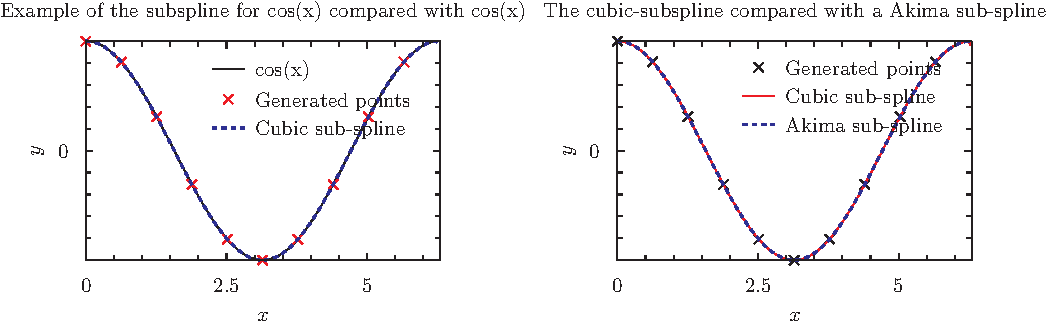
\includegraphics{cos.pdf}
\caption{A plot of a cos function and its derivitve. There is two sub-splines for the cos(x) points, a cubic sub-spline and Akima sub-spline.}
\end{center}
\end{figure}

As can be seen here both my cubic sub-spline and the Akima sub-spline fit the simple cos(x) points well and do a good job as splines without any wiggles.

\section{derivitive and integral}
Once this was done I found the derivitive and integral of the spline.

\begin{thebibliography}{H}
\bibitem{Dmitri} Fedorov, D.V. (2021), "Introduction to numerical methods",
\end{thebibliography}

\end{document}
